\documentclass[aspectratio=169,10pt]{beamer}
\usepackage[utf8]{inputenc}
\usepackage[T1]{fontenc}
\usepackage[brazil]{babel}
\usepackage{amsmath,amssymb}
\usepackage{booktabs}
\usepackage{array}
\usepackage{graphicx}
\usepackage{xcolor}
\usepackage{tikz}
\usepackage{siunitx}
\usetheme{Madrid}
\usecolortheme{default}
\setbeamertemplate{navigation symbols}{}
\setbeamertemplate{caption}[numbered]
\setbeamerfont{caption}{size=\scriptsize}
\setbeamerfont{frametitle}{size=\large}
\graphicspath{{../}}

\title[LLMs via Otimiza\c{c}\~ao Inversa]{Explicando Decis\~oes de LLMs via Otimiza\c{c}\~ao Inversa}
\subtitle{Disserta\c{c}\~ao de Mestrado}
\author{George Gomes da Silva}
\institute{Programa de P\'os-Gradua\c{c}\~ao em Inform\'atica}
\date{Abril de 2026}

\begin{document}

% ============ SLIDE 1 ============
\begin{frame}
  \titlepage
\end{frame}

% ============ SLIDE 2 ============
\begin{frame}{Motiva\c{c}\~ao}
  \textbf{Problema:} LLMs s\~ao caixas-pretas --- tomam decis\~oes sem explicar por qu\^e.
  \medskip

  \textbf{Pergunta central da disserta\c{c}\~ao:}
  \begin{quote}
    \emph{LLMs possuem um processo decis\'orio est\'avel e aprend\'ivel?}
  \end{quote}

  \textbf{Relev\^ancia:}
  \begin{itemize}
    \item \textbf{Explainability} --- auditoria de decis\~oes automatizadas.
    \item \textbf{Confiabilidade} --- mesmo crit\'erio em situa\c{c}\~oes diferentes?
    \item \textbf{Transfer\^encia de conhecimento} --- se h\'a um crit\'erio aprend\'ivel, ele pode ser extra\'ido, reutilizado e comparado.
    \item \textbf{Regula\c{c}\~ao} --- IA em \'areas cr\'iticas (sa\'ude, justi\c{c}a, cr\'edito) exige crit\'erios vers\'atil e inspecion\'aveis.
  \end{itemize}
\end{frame}

% ============ SLIDE 3 ============
\begin{frame}{Hip\'oteses}
  \small
  \begin{description}
    \item[\textbf{H1 --- Consist\^encia.}] O LLM mant\'em o mesmo crit\'erio decis\'orio impl\'icito. A m\'etrica $\hat{W}_{\text{LLM}}$ estimada prev\^e classifica\c{c}\~oes nos Problemas B e C.
    \item[\textbf{H2 --- Few-shot amplifica.}] Exemplos rotulados pela m\'etrica aumentam a concord\^ancia LLM--m\'etrica.
    \item[\textbf{H3 --- LLM como aprendiz.}] O LLM consegue aprender o crit\'erio de um perito externo via exemplos few-shot.
    \item[\textbf{H4 --- Exemplos dif\'iceis.}] Exemplos \emph{hard} (baixa margem) s\~ao mais informativos que \emph{easy}.
    \item[\textbf{H5 --- Estabilidade.}] Comportamento reprodut\'ivel entre execu\c{c}\~oes (m\'ultiplas seeds e repeti\c{c}\~oes).
  \end{description}
  \bigskip

  \emph{Nota:} H1--H3, H5 formuladas para confirma\c{c}\~ao; H4 testada como hip\'otese falsific\'avel.
\end{frame}

% ============ SLIDE 4 ============
\begin{frame}{Abordagem --- Otimiza\c{c}\~ao Inversa}
  \textbf{Intui\c{c}\~ao:} se o LLM tem crit\'erios est\'aveis, podemos aprender sua \emph{fun\c{c}\~ao objetivo impl\'icita} a partir das decis\~oes observadas.
  \medskip

  \textbf{M\'etrica de Mahalanobis diagonal:}
  \[
    d_W(x, c) = \sum_{j=1}^{d} w_j \cdot (x_j - c_j)^2, \quad w_j \geq 0
  \]

  \textbf{Classifica\c{c}\~ao nearest-centroid:}
  \[
    \hat{y}(x) = \arg\min_{k}\, d_W(x, c_k)
  \]
  \medskip

  \textbf{Otimiza\c{c}\~ao inversa:} dado $\{(x_i, y_i^{\text{LLM}})\}$, inferir $W$ tal que essas rotula\c{c}\~oes sejam \'otimas sob $d_W$. Framework de Ahuja \& Orlin (2001).
\end{frame}

% ============ SLIDE 5 ============
\begin{frame}{Vis\~ao Geral dos Dados Sint\'eticos 2D}
  \textbf{4 problemas} gerados com \texttt{sklearn.datasets.make\_blobs}.
  \begin{center}
    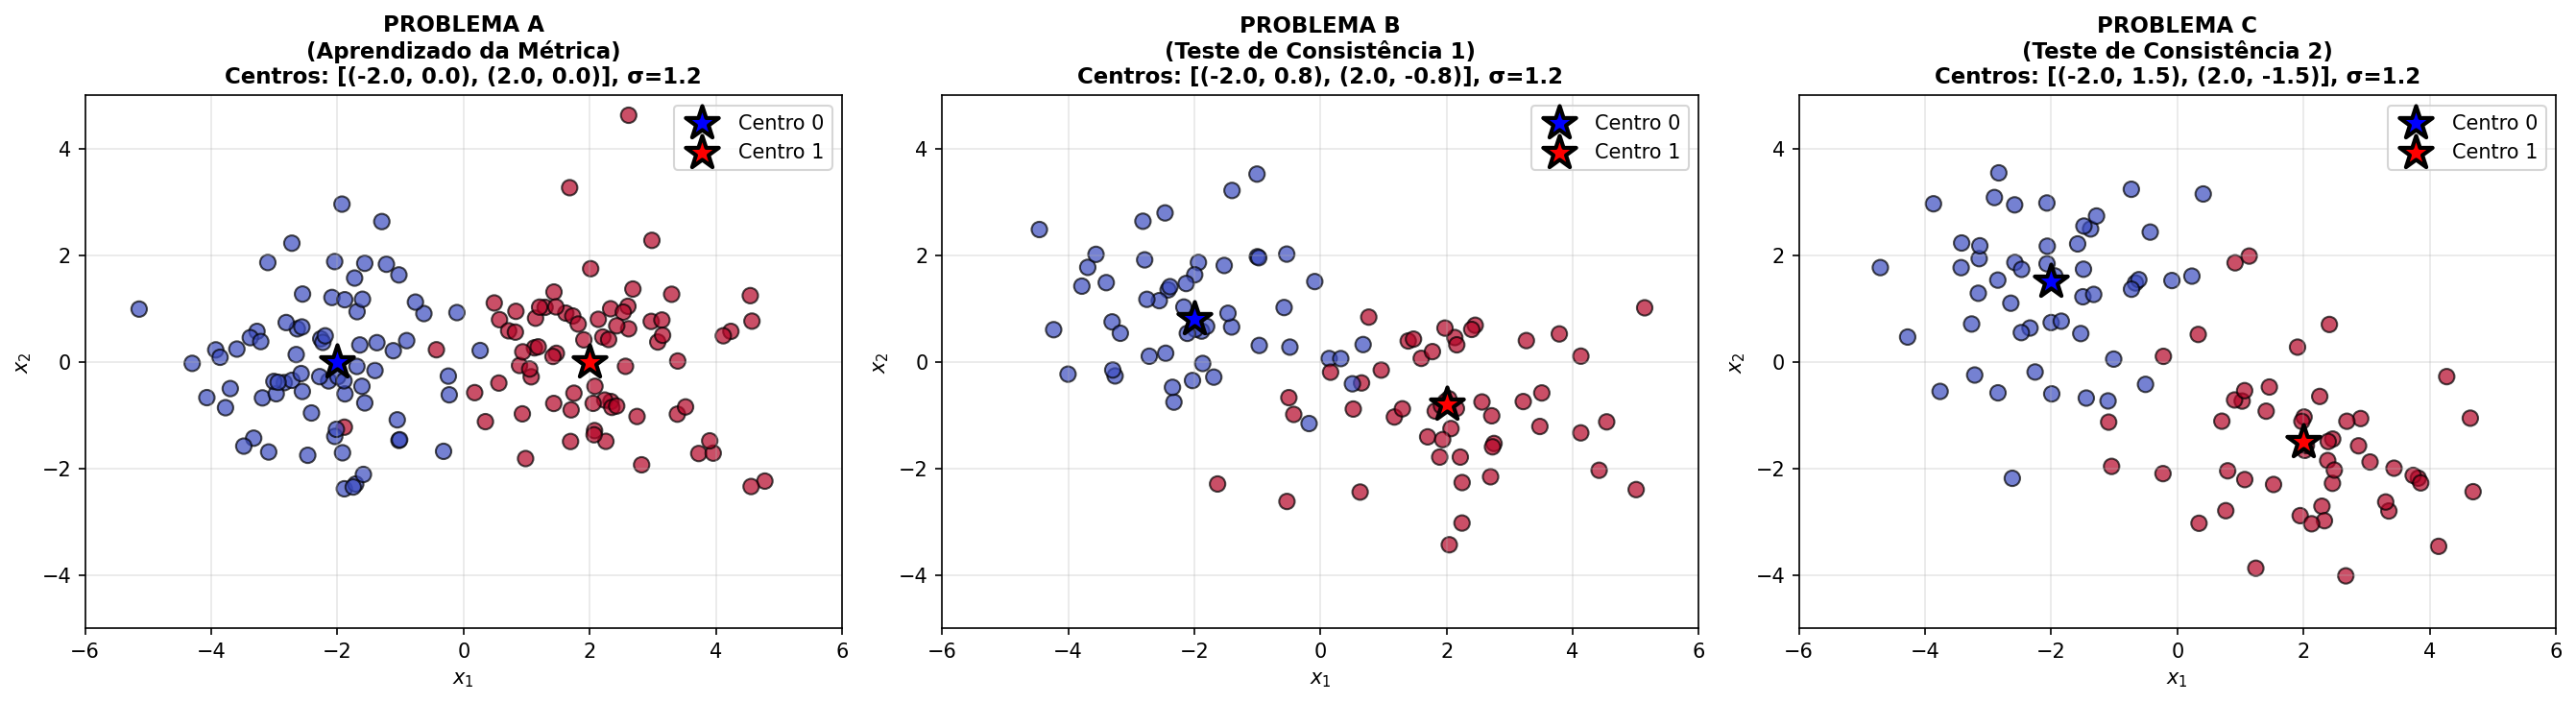
\includegraphics[width=0.92\linewidth,height=0.72\textheight,keepaspectratio]{01_all_three_problems.png}
  \end{center}
  \scriptsize Problemas A (treino da m\'etrica), B e C (testes de consist\^encia). O Problema D (Fase D) tem perito externo com m\'etrica conhecida.
\end{frame}

% ============ SLIDE 6 ============
\begin{frame}{Problema A --- Treino da M\'etrica}
  \footnotesize
  \textbf{Par\^ametros:}
  \begin{itemize}
    \item $n = 150$ amostras, 2 classes
    \item Centr\'oides: $c_0 = (-2, -0.5)$, $c_1 = (2, 0.5)$
    \item $\texttt{cluster\_std} = 1.2$
    \item Seeds: \{42, 123, 7\}
  \end{itemize}
  \vspace{-0.1cm}
  \begin{center}
    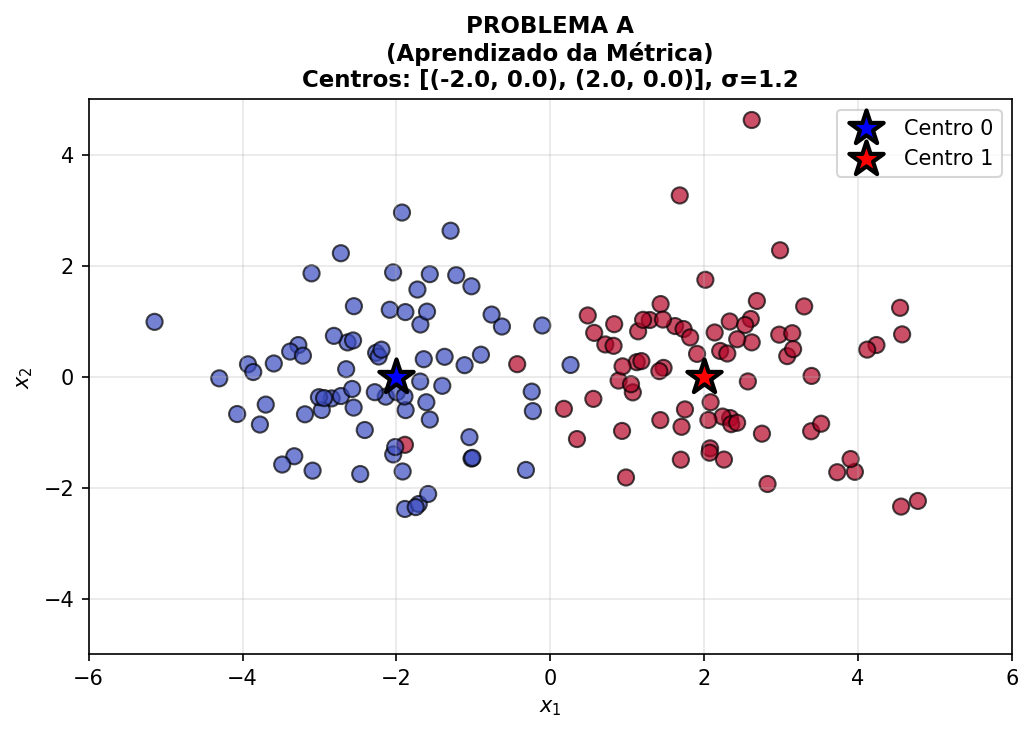
\includegraphics[width=0.75\linewidth,height=0.55\textheight,keepaspectratio]{01_all_three_problems_problema_a.png}
  \end{center}
\end{frame}

% ============ SLIDE 7 ============
\begin{frame}{Problema B --- Teste de Consist\^encia 1}
  \footnotesize
  \textbf{Par\^ametros:}
  \begin{itemize}
    \item $n = 100$ amostras, 2 classes
    \item Centr\'oides deslocados \emph{verticalmente} (geometria distinta de A)
    \item $\texttt{cluster\_std} = 1.2$
  \end{itemize}
  \vspace{-0.1cm}
  \begin{center}
    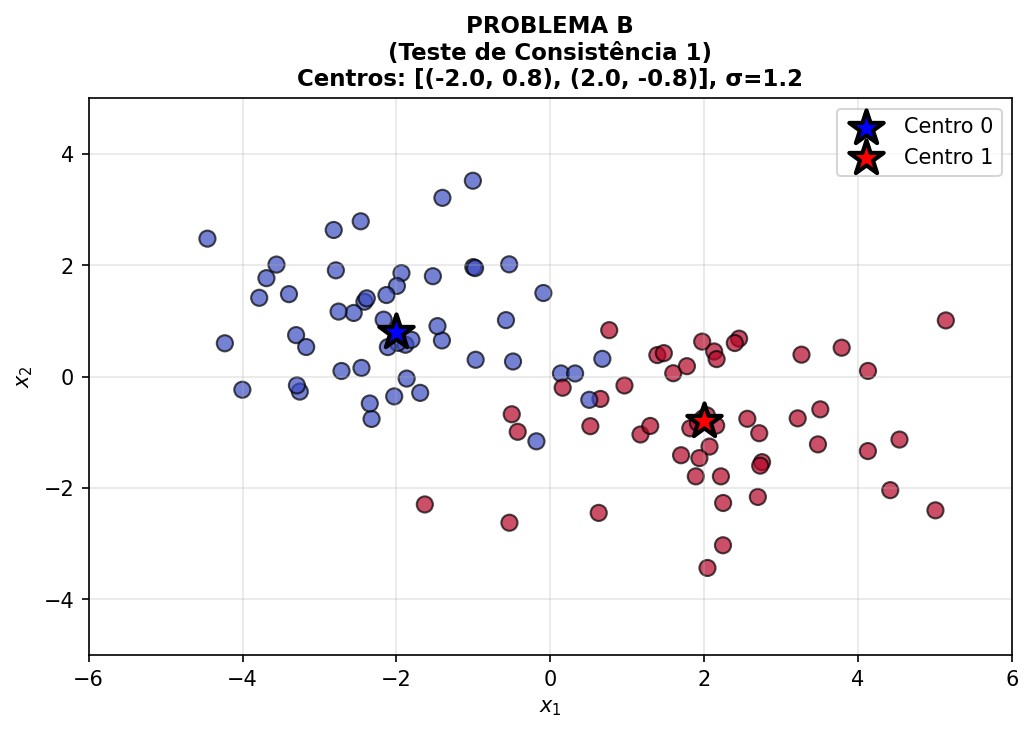
\includegraphics[width=0.75\linewidth,height=0.55\textheight,keepaspectratio]{01_all_three_problems_problema_b.png}
  \end{center}
\end{frame}

% ============ SLIDE 8 ============
\begin{frame}{Problema C --- Teste de Consist\^encia 2}
  \footnotesize
  \textbf{Par\^ametros:}
  \begin{itemize}
    \item $n = 100$ amostras
    \item Distor\c{c}\~ao geom\'etrica \emph{mais severa} (escala e orienta\c{c}\~ao alteradas)
    \item $\texttt{cluster\_std}$ maior, separa\c{c}\~ao n\~ao paralela aos eixos
  \end{itemize}
  \vspace{-0.1cm}
  \begin{center}
    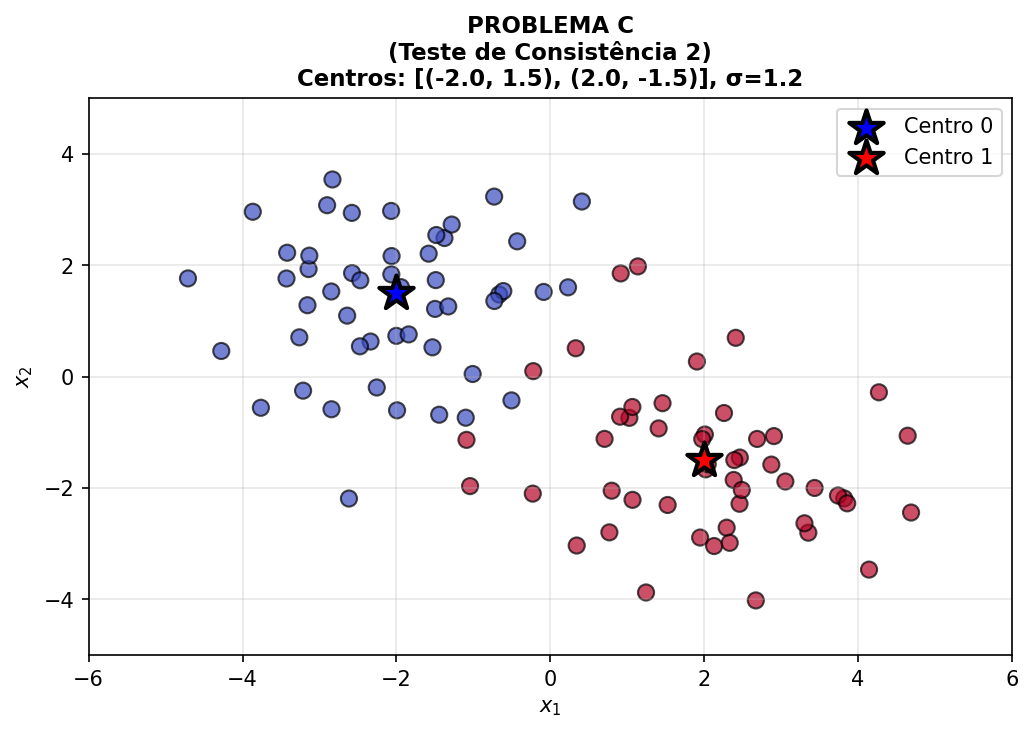
\includegraphics[width=0.75\linewidth,height=0.55\textheight,keepaspectratio]{01_all_three_problems_problema_c.png}
  \end{center}
\end{frame}

% ============ SLIDE 9 ============
\begin{frame}{Problema D --- Perito Externo}
  \footnotesize
  \textbf{Par\^ametros:}
  \begin{itemize}
    \item $n = 150$; perito rotula com $W_{\text{expert}} = [0.3,\, 1.5]$ (pondera $x_2$ $5\times$ mais que $x_1$)
    \item Centr\'oides: $(-1.5, 1.0)$ e $(1.5, -1.0)$
  \end{itemize}
  \vspace{-0.1cm}
  \begin{center}
    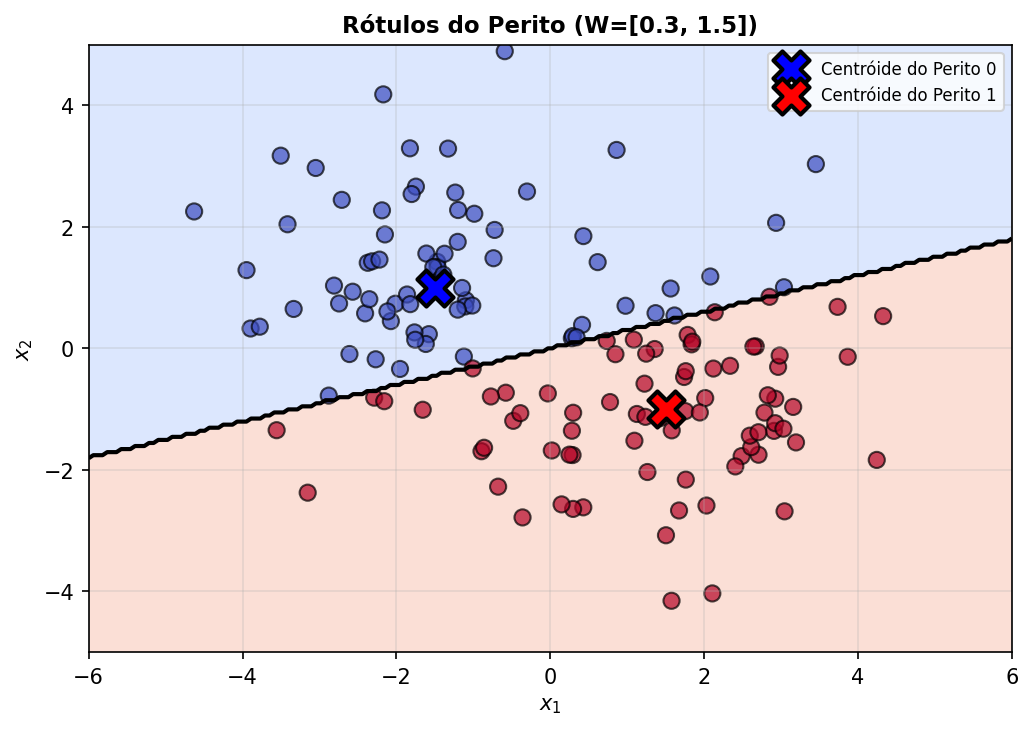
\includegraphics[width=0.8\linewidth,height=0.55\textheight,keepaspectratio]{06_problem_d_expert_fronteira_perito.png}
  \end{center}
  \scriptsize Fronteira do perito (linha s\'olida) --- LLM deve \emph{aprender} esse crit\'erio via few-shot.
\end{frame}

% ============ SLIDE 10 ============
\begin{frame}{Configura\c{c}\~oes de Execu\c{c}\~ao}
  \footnotesize
  \begin{center}
  \begin{tabular}{ll}
    \toprule
    \textbf{Configura\c{c}\~ao} & \textbf{Valor} \\
    \midrule
    Modelo LLM & gpt-4o-mini (OpenAI), temperatura $0.0$ \\
    Seeds aleat\'orias & $\{42,\, 123,\, 7\}$ \\
    Repeti\c{c}\~oes por config & $3$ \\
    Few-shot (Fases B/C) & $\{0, 5, 10, 20, 40\}$ \\
    Few-shot (Fase D) & $\{0, 5, 10, 20, 40\}$ \\
    Concorr\^encia ass\'incrona & \texttt{asyncio.Semaphore(10)} \\
    Nomes de classe (viés) & \{A/B, 0/1, Positivo/Negativo, Azul/Vermelho\} + inversos \\
    Estrat\'egias (Fase D) & \{easy, hard, mixed, random\} \\
    Experts (Fase D) & \{aniso\_x2, aniso\_x1, euclidean\} \\
    Variantes de prompt & \{default, geometric, cot, tabular\} \\
    Total de chamadas ao LLM & $114.478$ \\
    \bottomrule
  \end{tabular}
  \end{center}
\end{frame}

% ============ SLIDE — Por que múltiplas seeds? (NOVO) ============
\begin{frame}{Por que m\'ultiplas seeds?}
  \footnotesize
  \textbf{3 sementes} (42, 123, 7) $\times$ \textbf{3 repeti\c{c}\~oes} por configura\c{c}\~ao.
  \medskip

  \begin{enumerate}
    \item \textbf{Estocasticidade dos dados:} \texttt{make\_blobs} usa amostras aleat\'orias --- uma \'unica seed pode produzir geometria at\'ipica.
    \item \textbf{Estocasticidade residual do LLM:} mesmo com temperatura $0$, batching em GPU e top-$k$ produzem varia\c{c}\~ao entre chamadas.
    \item \textbf{Inferência estat\'istica:} m\'ultiplas seeds permitem
      \begin{itemize}
        \item bootstrap 95\% CI (10k reamostragens);
        \item teste de reprodutibilidade (H5);
        \item descartar achados dependentes de seed espec\'ifica.
      \end{itemize}
    \item \textbf{Pr\'atica padr\~ao em ML emp\'irico:} evita ``p-hacking de seed'' (Bouthillier et al., 2021).
  \end{enumerate}
  \medskip

  \textbf{Resultado esperado:} dire\c{c}\~ao de $W$ (raz\~ao $w_1/w_2$) e fidelidade devem ser \emph{qualitativamente est\'aveis} entre seeds.
\end{frame}

% ============ SLIDE 11 ============
\begin{frame}{Algoritmo 1 --- Perceptron Estruturado (pseudo-c\'odigo completo)}
  \scriptsize
  \textbf{Formula\c{c}\~ao (Coelho, Borges \& Fonseca Neto, CILAMCE 2017, Eq.~28):}
  \[
    \max_{\gamma}\; \gamma \quad\text{s.t.}\quad
    \underbrace{\sum_j w_j [(x_{ij}-c_{kj})^2 - (x_{ij}-c_{\ell j})^2]}_{\text{margem}_i(W)} + \lambda \alpha_i \geq \gamma \cdot \|w\|,\; w \geq 0
  \]

  \textbf{Algoritmo (busca bin\'aria + perceptron interno):}
  \begin{enumerate}
    \item Inicializar $w \leftarrow \mathbf{1}$, $\gamma_{\text{lo}} \leftarrow 0$, $\gamma_{\text{hi}} \leftarrow \infty$, $\gamma \leftarrow \gamma_{\text{init}}$.
    \item \textbf{Loop externo} (busca bin\'aria em $\gamma$):
      \begin{enumerate}
        \item \textbf{Loop interno} (perceptron multiplicativo) por $\text{max\_iter}$ \'epocas:
        \begin{itemize}
          \item Para cada $i$ com $\text{margem}_i(W) < \gamma$: $w \leftarrow w + \eta \cdot [(x_i - c_k)^2 - (x_i - c_\ell)^2]$; projetar $w \geq 0$.
        \end{itemize}
        \item Se $\text{viola\c{c}\~oes} = 0$: salvar $w^\star$; $\gamma_{\text{lo}} \leftarrow \gamma$; $\gamma \leftarrow \gamma + \Delta\gamma$.
        \item Sen\~ao: $\gamma_{\text{hi}} \leftarrow \gamma$; $\gamma \leftarrow (\gamma_{\text{lo}} + \gamma_{\text{hi}})/2$ (bisse\c{c}\~ao); restaurar $w^\star$.
        \item Parar quando $|\gamma_{\text{hi}} - \gamma_{\text{lo}}| \leq \text{tol}$.
      \end{enumerate}
  \end{enumerate}

  \textbf{Hiperpar\^ametros:} $\eta = 1$ (padr\~ao), $C = 10$, $\Delta\gamma = 0.05$, $\text{max\_iter} = 50$, $\text{tol} = 10^{-4}$.
\end{frame}

% ============ SLIDE 12 ============
\begin{frame}{Algoritmo 2 --- NNLS (M\'inimos Quadrados, pseudo-c\'odigo completo)}
  \scriptsize
  \textbf{Formula\c{c}\~ao:} resolver o sistema sobredeterminado $A\,w \approx b$ sob restri\c{c}\~ao de positividade.
  \[
    \min_{W}\, \|A\,w - b\|^2 \quad \text{sujeito a}\quad w_j \geq 0
  \]

  \textbf{Pseudo-c\'odigo:}
  \begin{enumerate}
    \item Para cada ponto $x_i$ com classe correta $c_{\ell}$ e rival $c_k$:
      \begin{itemize}
        \item $A_i \leftarrow (x_i - c_k)^2 - (x_i - c_{\ell})^2 \quad$ (vetor de tamanho $d$).
        \item $b_i \leftarrow \text{target\_margin} = 1$ (margem-alvo constante).
      \end{itemize}
    \item Empilhar $A \in \mathbb{R}^{n \times d}$ e $b \in \mathbb{R}^n$.
    \item Chamar \texttt{w, residual = scipy.optimize.nnls(A, b)}.
    \item (opcional) Normalizar $w \leftarrow w / \|w\|$ para visualiza\c{c}\~ao.
  \end{enumerate}

  \textbf{Garantia:} $w \geq 0$ por constru\c{c}\~ao (m\'etrica diagonal semidefinida positiva). \'Otimo \'unico em problemas bem-condicionados (Lawson \& Hanson, 1974).
  \medskip

  \textbf{Vantagem:} zero hiperpar\^ametros $\Rightarrow$ resultado totalmente determin\'istico, independe de inicializa\c{c}\~ao.
  \medskip

  \textbf{Justificativa de $\text{target\_margin}=1$:} a raz\~ao $w_1/w_2$ (que determina a fronteira) \'e invariante \`a escala de $b$.
\end{frame}

% ============ SLIDE 14 ============
\begin{frame}{Robustez da Coleta de Decis\~oes do LLM}
  \footnotesize
  \textbf{Pipeline de chamada ao LLM:}
  \begin{enumerate}
    \item \textbf{Parser de 7 camadas} (\texttt{parse\_llm\_response}): extra\c{c}\~ao por resposta limpa, \texttt{startswith}, regex, busca de palavra inteira, fuzzy matching, \dots
    \item \textbf{Retentativas:} \texttt{MAX\_FORMAT\_RETRIES = 5} --- se a resposta for malformada, reenvia o prompt com instru\c{c}\~ao refor\c{c}ada.
    \item \textbf{Fallback determin\'istico por hash MD5:} ap\'os 5 falhas, r\'otulo = $\text{MD5}(x_1, x_2) \bmod 2$. Substitui aritm\'etica modular direta para n\~ao introduzir vi\'es geom\'etrico.
    \item \textbf{Concorr\^encia ass\'incrona:} \texttt{asyncio.Semaphore(10)} permite at\'e 10 chamadas paralelas $\Rightarrow$ redu\c{c}\~ao de $\sim 10\times$ no tempo de coleta.
  \end{enumerate}
  \bigskip

  \textbf{Observa\c{c}\~ao:} temperatura $0.0$ \emph{n\~ao} garante determinismo (batching em GPU, top-$k$ residual, hardware heterog\^eneo). M\'ultiplas seeds e repeti\c{c}\~oes s\~ao \textbf{essenciais}.
\end{frame}

% ============ SLIDE 15 ============
\begin{frame}{Fase A --- Descri\c{c}\~ao}
  \textbf{Objetivo:} capturar o processo decis\'orio \emph{intr\'inseco} do LLM.
  \medskip

  \textbf{Protocolo:}
  \begin{enumerate}
    \item LLM classifica 150 pontos do Problema A \textbf{zero-shot} (sem exemplos).
    \item Centr\'oides $\hat{c}_k$ s\~ao recalculados a partir das decis\~oes do LLM.
    \item Cada algoritmo de otimiza\c{c}\~ao inversa (Perceptron, NNLS) estima um $W$ independente a partir dessas decis\~oes.
    \item \textbf{Fidelidade:} $\%$ das decis\~oes do LLM que a m\'etrica aprendida reproduz.
  \end{enumerate}
  \medskip

  \textbf{Por que zero-shot?} isola o \emph{vi\'es intr\'inseco} do modelo, sem contamina\c{c}\~ao de exemplos.
\end{frame}

% ============ SLIDE 16 ============
\begin{frame}{Fase A --- W Aprendido e Fidelidade}
  \footnotesize
  \textbf{M\'edias (Fase A, classes A/B, zero-shot, 3 seeds $\times$ 3 reps):}
  \begin{center}
  \begin{tabular}{lccc}
    \toprule
    \textbf{Algoritmo} & $\hat{W}$ unit\'ario t\'ipico (seed 42) & \textbf{Raz\~ao} $w_1/w_2$ & \textbf{Fid.~Prob.~A} \\
    \midrule
    Perceptron & $[0.39,\, 0.92]$ & $0.43$ & $81.3\%$ \\
    NNLS       & $[0.20,\, 0.80]$ & $0.25$ & $84.7\%$ \\
    \bottomrule
  \end{tabular}
  \end{center}
  \vspace{-0.15cm}
  \begin{center}
    
\includegraphics[width=0.65\linewidth,height=0.46\textheight,keepaspectratio]{11_metric_errors_phase_a_seed42_mapa_erros.png}
  \end{center}
  \scriptsize Mapa de erros da m\'etrica (seed 42): pontos vermelhos = onde a m\'etrica discorda do LLM.
\end{frame}

% ============ SLIDE 17 ============
\begin{frame}{Fase A --- An\'alise Quantitativa de Erros por Regi\~ao}
  \scriptsize
  \textbf{Decomposi\c{c}\~ao dos erros da m\'etrica por dist\^ancia \`a fronteira (seed 42):}
  \begin{center}
  \begin{tabular}{lrrrr}
    \toprule
    \textbf{Regi\~ao} & \textbf{N pontos} & \textbf{Erros} & \textbf{Taxa erro} & \textbf{\% dos erros} \\
    \midrule
    Baixa margem (fronteira) & 50 & 20 & $40.0\%$ & $74.1\%$ \\
    Margem m\'edia           & 49 &  6 & $12.2\%$ & $22.2\%$ \\
    Alta margem (longe)      & 51 &  1 & $2.0\%$  & $3.7\%$ \\
    \bottomrule
  \end{tabular}
  \end{center}
  \medskip

  \textbf{Testes de significância (seed 42):}
  \begin{itemize}
    \item Correla\c{c}\~ao ponto-bisserial (acerto $\times$ margem): $r = 0.395$, $p < 0.001$
    \item Mann-Whitney U (margem de acertos $>$ margem de erros): $U = 2708$, $p < 0.001$
    \item Margem m\'edia dos acertos: $4.51$ vs.\ erros: $1.97$
  \end{itemize}
  \medskip

  \textbf{Resultado consistente entre seeds:} seeds 7, 42, 123 todas confirmam que $\geq 65\%$ dos erros concentram-se pr\'oximos \`a fronteira.
\end{frame}

% ============ SLIDE 18 ============
\begin{frame}{Fase A --- Distribui\c{c}\~ao de W entre Seeds}
  \begin{center}
    
\includegraphics[width=0.78\linewidth,height=0.68\textheight,keepaspectratio]{10_w_distribution_boxplot.png}
  \end{center}
  \footnotesize
  \textbf{Dire\c{c}\~ao de $W$ est\'avel:} cosseno m\'edio entre seeds $= 0.984$, range $[0.975, 0.992]$.
  \textbf{Raz\~ao $w_1/w_2$:} m\'edia $0.405$, CI$_{95}$ $[0.318, 0.458]$, CV $= 32\%$ em zero-shot, cai para $6\%$ com few-shot $\geq 5$.
\end{frame}

% ============ SLIDE 19 ============
\begin{frame}{Fase A --- Compara\c{c}\~ao dos 2 Algoritmos}
  \begin{center}
    
\includegraphics[width=0.95\linewidth,height=0.68\textheight,keepaspectratio]{14_algorithm_comparison_fidelidade.png}
  \end{center}
  \footnotesize
  \textbf{Similaridade de cosseno entre algoritmos (zero-shot):}
  \begin{itemize}
    \item Perceptron $\leftrightarrow$ NNLS: $0.986$
  \end{itemize}
  Os 2 algoritmos convergem para m\'etricas \emph{geometricamente similares} --- resultado robusto ao m\'etodo de estima\c{c}\~ao.
\end{frame}

% ============ SLIDE 20 ============
\begin{frame}{Fase A --- Sensibilidade a Hiperpar\^ametros do Perceptron}
  \scriptsize
  \textbf{Re-execu\c{c}\~ao do Perceptron com configs (seed 7), sem nova chamada ao LLM:}
  \begin{center}
  \begin{tabular}{lcccc}
    \toprule
    \textbf{Varia\c{c}\~ao} & \textbf{Valor} & $\hat{W}$ unit\'ario & $\cos(\text{default})$ & \textbf{Fid.} \\
    \midrule
    $\eta$ (padr\~ao $0.05$) & $0.01$ & $[0.79, 0.61]$ & $0.896$ & $74.7\%$ \\
                             & $0.10$ & $[0.35, 0.94]$ & $0.996$ & $82.7\%$ \\
                             & $0.50$ & $[0.00, 1.00]$ & $0.900$ & $79.3\%$ \\
    \midrule
    $C$ (padr\~ao $10$)      & $1.0$  & $[0.23, 0.97]$ & $0.977$ & $86.0\%$ \\
                             & $50$   & $[0.77, 0.64]$ & $0.911$ & $74.7\%$ \\
    \midrule
    $\delta_\gamma$ (padr\~ao $0.05$) & $0.01$ & $[0.36, 0.93]$ & $0.996$ & $82.7\%$ \\
                                       & $0.10$ & $[0.55, 0.84]$ & $0.992$ & $78.7\%$ \\
    \bottomrule
  \end{tabular}
  \end{center}
  \medskip

  \textbf{Conclus\~ao:} $\cos \geq 0.86$ em todas as configs (3 seeds) $\Rightarrow$ \emph{W moderadamente sens\'ivel}, mas a \emph{dire\c{c}\~ao} (que determina a fronteira) \'e est\'avel. NNLS (sem hiperpar\^ametros) serve como refer\^encia.
\end{frame}

% ============ SLIDE 21 ============
\begin{frame}{Fases B e C --- Descri\c{c}\~ao}
  \textbf{Pergunta central:} $\hat{W}_{\text{LLM}}$ (aprendido em A) generaliza para novos problemas?
  \medskip

  \textbf{Protocolo:}
  \begin{enumerate}
    \item Aplicar $\hat{W}_{\text{LLM}}$ (da Fase A) e centr\'oides locais dos Problemas B e C.
    \item Coletar decis\~oes do LLM nos mesmos pontos.
    \item Comparar.
  \end{enumerate}
  \medskip

  \textbf{M\'etricas reportadas:}
  \begin{itemize}
    \item Consist\^encia (\% concord\^ancia LLM vs.\ m\'etrica)
    \item Kappa de Cohen (concord\^ancia corrigida pelo acaso)
    \item F1-Score (m\'edia ponderada por classe)
  \end{itemize}
\end{frame}

% ============ SLIDE 22 ============
\begin{frame}{Fases B e C --- Resultados (1/2)}
  \scriptsize
  \textbf{Consist\^encia por \texttt{n\_shot} (todas as variantes de classe, default prompt):}
  \begin{center}
  \begin{tabular}{rcccc}
    \toprule
    $\mathbf{n\_shot}$ & \textbf{Consist.~B} & \textbf{Consist.~C} & \textbf{Kappa B} & \textbf{Kappa C} \\
    \midrule
    0  & $66.7\% \pm 9.7\%$ & $66.7\% \pm 8.4\%$ & $0.189$ & $0.215$ \\
    5  & $80.0\% \pm 1.5\%$ & $79.5\% \pm 8.3\%$ & $0.598$ & $0.570$ \\
    10 & $83.7\% \pm 9.9\%$ & $81.2\% \pm 15.5\%$ & $0.629$ & $0.614$ \\
    20 & $83.9\% \pm 11.5\%$ & $71.0\% \pm 12.1\%$ & $0.671$ & $0.413$ \\
    40 & $74.6\% \pm 9.2\%$ & $69.6\% \pm 12.3\%$ & $0.492$ & $0.395$ \\
    \bottomrule
  \end{tabular}
  \end{center}
  \medskip

  \textbf{Consist\^encia m\'edia agregada:} Problema B $= 78.2\% \pm 12.1\%$; Problema C $= 75.6\% \pm 14.5\%$.
\end{frame}

% ============ SLIDE 23 ============
\begin{frame}{Fases B e C --- Resultados (2/2)}
  \begin{center}
    
\includegraphics[width=0.92\linewidth,height=0.8\textheight,keepaspectratio]{02_consistency_extended_consistencia.png}
  \end{center}
\end{frame}

% ============ SLIDE 24 ============
\begin{frame}{Fases B e C --- Discuss\~ao}
  \footnotesize
  \textbf{Interpreta\c{c}\~ao de Kappa (Landis \& Koch, 1977):}
  \begin{itemize}
    \item $[0.41, 0.60]$: concord\^ancia moderada --- observada em zero-shot e $n \geq 20$
    \item $[0.61, 0.80]$: concord\^ancia substancial --- observada em $n \in \{5, 10\}$
  \end{itemize}
  \medskip

  \textbf{H1 (consist\^encia):} \emph{parcialmente confirmada}. O LLM mant\'em $W$ est\'avel na \emph{dire\c{c}\~ao} entre seeds, mas a fidelidade da m\'etrica no Problema A cai conforme a geometria de B/C se distancia de A.
  \medskip

  \textbf{Observa\c{c}\~ao curiosa:} consist\^encia \emph{decai} para $n=40$ em ambos problemas. Hip\'otese: com muitos exemplos, o LLM pode come\c{c}ar a interpolar entre eles em vez de seguir um crit\'erio consistente, aproximando-se do vi\'es dos pr\'oprios exemplos.
  \medskip

  \textbf{M\'etrica estimada vs.\ Euclidiana (zero-shot, B):} $\Delta = +14.8\%$, CI$_{95}$ $[+3.5\%, +30.4\%]$ $\Rightarrow$ \textbf{m\'etrica significativamente melhor}.
\end{frame}

% ============ SLIDE 25 ============
\begin{frame}{Vi\'es de Ordem das Classes}
  \scriptsize
  \textbf{Consist\^encia m\'edia ($n=10$) por ordena\c{c}\~ao de r\'otulos:}
  \begin{center}
  \begin{tabular}{lcc}
    \toprule
    \textbf{Ordem} & \textbf{Consist.~B} & \textbf{Consist.~C} \\
    \midrule
    A/B           & $81.0\%$ & $67.7\%$ \\
    B/A (inverso) & $91.5\%$ & $93.5\%$ \\
    0/1           & $85.9\%$ & $77.6\%$ \\
    1/0 (inverso) & $80.4\%$ & $88.5\%$ \\
    Azul/Vermelho & $84.3\%$ & $84.3\%$ \\
    Vermelho/Azul (inverso) & $89.8\%$ & $95.1\%$ \\
    \bottomrule
  \end{tabular}
  \end{center}
  \medskip

  \textbf{Achado:} inverter a ordem das classes no prompt \textbf{altera} o desempenho em at\'e $25$ p.p.\ (A/B $\to$ B/A). O LLM tem \emph{vi\'es de posi\c{c}\~ao} na enumera\c{c}\~ao de classes.
\end{frame}

% ============ SLIDE 26 ============
\begin{frame}{Vi\'es de Ordem das Classes --- Gr\'afico}
  \begin{center}
    
\includegraphics[width=0.95\linewidth,height=0.82\textheight,keepaspectratio]{15_class_order_bias_consistencia.png}
  \end{center}
\end{frame}

% ============ SLIDE 27 ============
\begin{frame}{Nomes Sem\^anticos de Features}
  \footnotesize
  \textbf{Efeito de nomes semânticos (zero-shot, 3 seeds):}
  \begin{center}
  \begin{tabular}{lcc}
    \toprule
    \textbf{Nomes das features} & \textbf{Fid.~A} & \textbf{Consist.~B} \\
    \midrule
    \texttt{x1 / x2}               (neutro) & $72.8\%$ & $66.9\%$ \\
    \texttt{altura / peso}         (sem\^antico) & $84.0\%$ & $74.0\%$ \\
    \texttt{feature\_1 / feature\_2} (t\'ecnico) & $58.0\%$ & $54.0\%$ \\
    \bottomrule
  \end{tabular}
  \end{center}
  \medskip

  \textbf{Achado:}
  \begin{itemize}
    \item Nomes sem\^anticos (altura/peso) aumentam a fidelidade em \textbf{+11 p.p.}
    \item Nomes gen\'ericos (feature\_1/feature\_2) \textbf{reduzem} a fidelidade em \textbf{-14 p.p.}
    \item O LLM est\'a sens\'ivel \`a \emph{semântica} do nome --- n\~ao apenas \`a distribui\c{c}\~ao num\'erica.
  \end{itemize}
\end{frame}

% ============ SLIDE 28 ============
\begin{frame}{Variantes de Prompt (1/2) --- Design}
  \footnotesize
  \textbf{4 variantes testadas nas Fases A-C em todas as seeds:}
  \begin{description}
    \item[\texttt{default}] Template padr\~ao (baseline): coordenadas num\'ericas, pergunta direta.
    \item[\texttt{geometric}] Contexto \emph{geom\'etrico} expl\'icito: \emph{``considere cada ponto em um plano 2D''}.
    \item[\texttt{cot}] \emph{Chain-of-thought}: instrui raciocinar passo a passo antes de responder.
    \item[\texttt{tabular}] Coordenadas apresentadas como tabela markdown.
  \end{description}
  \medskip

  \textbf{Protocolo:} Fases A-C completas em todas as seeds para cada variante. Se $\hat{W}$ mudar entre variantes $\Rightarrow$ o prompt \emph{confunde a medi\c{c}\~ao} (vi\'es de formula\c{c}\~ao).
\end{frame}

% ============ SLIDE 29 ============
\begin{frame}{Variantes de Prompt (2/2) --- Resultados}
  \scriptsize
  \textbf{Fase A (zero-shot), m\'edia sobre 3 seeds:}
  \begin{center}
  \begin{tabular}{lccc}
    \toprule
    \textbf{Variante} & \textbf{Fid.~A} & \textbf{Consist.~B} & \textbf{Consist.~C} \\
    \midrule
    \texttt{default}   & $81.3\%$ & $72.4\%$ & $70.6\%$ \\
    \texttt{geometric} & $76.4\%$ & $\sim 75\%$ & $73.8\%$ \\
    \texttt{cot}       & $69.6\%$ & $\sim 68\%$ & $61.1\%$ \\
    \texttt{tabular}   & $61.6\%$ & $\sim 60\%$ & $60.6\%$ \\
    \bottomrule
  \end{tabular}
  \end{center}
  \vspace{-0.1cm}
  \begin{center}
    
\includegraphics[width=0.62\linewidth,height=0.45\textheight,keepaspectratio]{17_prompt_variant_comparison_fidelidade.png}
  \end{center}
  \scriptsize \emph{default} e \emph{geometric} s\~ao equivalentes; \emph{cot} degrada (raciocínio expl\'icito introduz ru\'ido); \emph{tabular} \'e o pior (formato compete com a tarefa).
\end{frame}

% ============ SLIDE 30 ============
\begin{frame}{Fase D --- Descri\c{c}\~ao}
  \footnotesize
  \textbf{Invers\~ao de pap\'eis:} agora o LLM \'e o \emph{aprendiz}.
  \begin{itemize}
    \item Perito externo com $W_{\text{expert}} = [0.3, 1.5]$ rotula os 150 pontos do Problema D.
    \item Acur\'acia do perito vs.\ ground-truth: $89.9\%$.
    \item LLM recebe $n \in \{0, 5, 10, 20, 40\}$ exemplos rotulados pelo perito (few-shot).
    \item LLM tenta \emph{aprender} o crit\'erio do perito e classificar o restante.
  \end{itemize}
  \vspace{-0.1cm}
  \begin{center}
    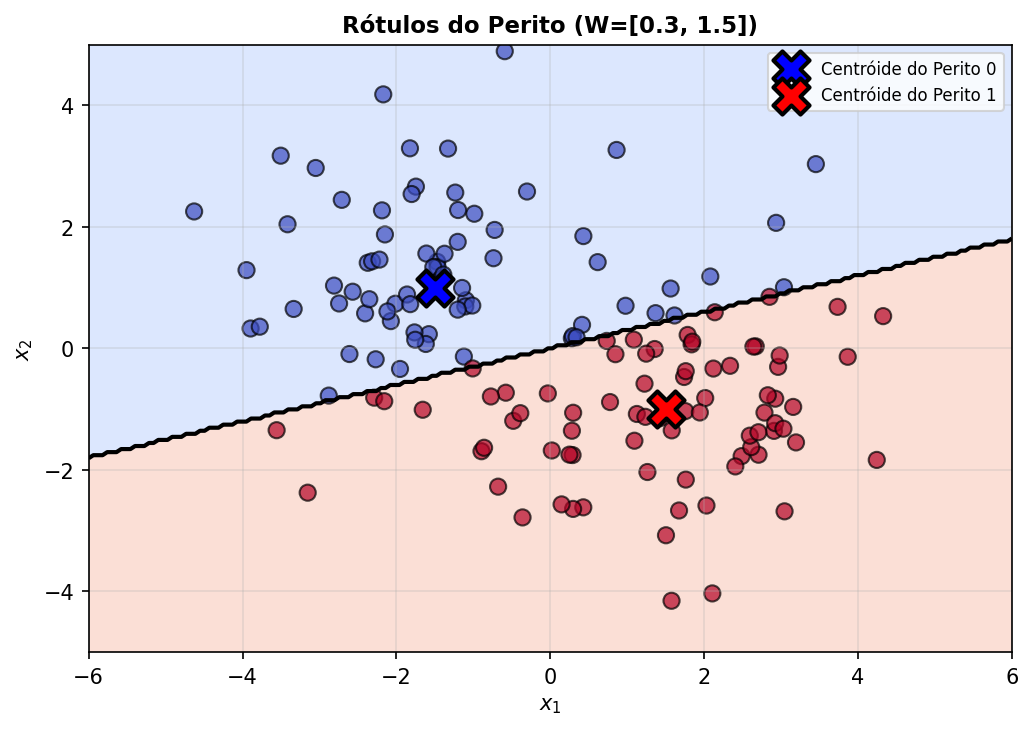
\includegraphics[width=0.55\linewidth,height=0.45\textheight,keepaspectratio]{06_problem_d_expert_fronteira_perito.png}
  \end{center}
  \scriptsize Linha s\'olida: fronteira do perito ($x_2 \approx 5\times$ mais importante que $x_1$).
\end{frame}

% ============ SLIDE 31 ============
\begin{frame}{Fase D --- Estrat\'egias de Sele\c{c}\~ao de Exemplos}
  \footnotesize
  \textbf{4 estrat\'egias} de sele\c{c}\~ao dos exemplos few-shot, balanceadas por classe:
  \begin{description}
    \item[\textbf{easy}] Pontos com \emph{alta margem} (longe da fronteira) --- prototípicos.
    \item[\textbf{hard}] Pontos com \emph{baixa margem} (próximos da fronteira) --- amb\'iguos.
    \item[\textbf{mixed}] 50\% easy + 50\% hard.
    \item[\textbf{random}] Sele\c{c}\~ao aleat\'oria balanceada (baseline sem estrat\'egia).
  \end{description}
  \vspace{-0.1cm}
  \begin{center}
    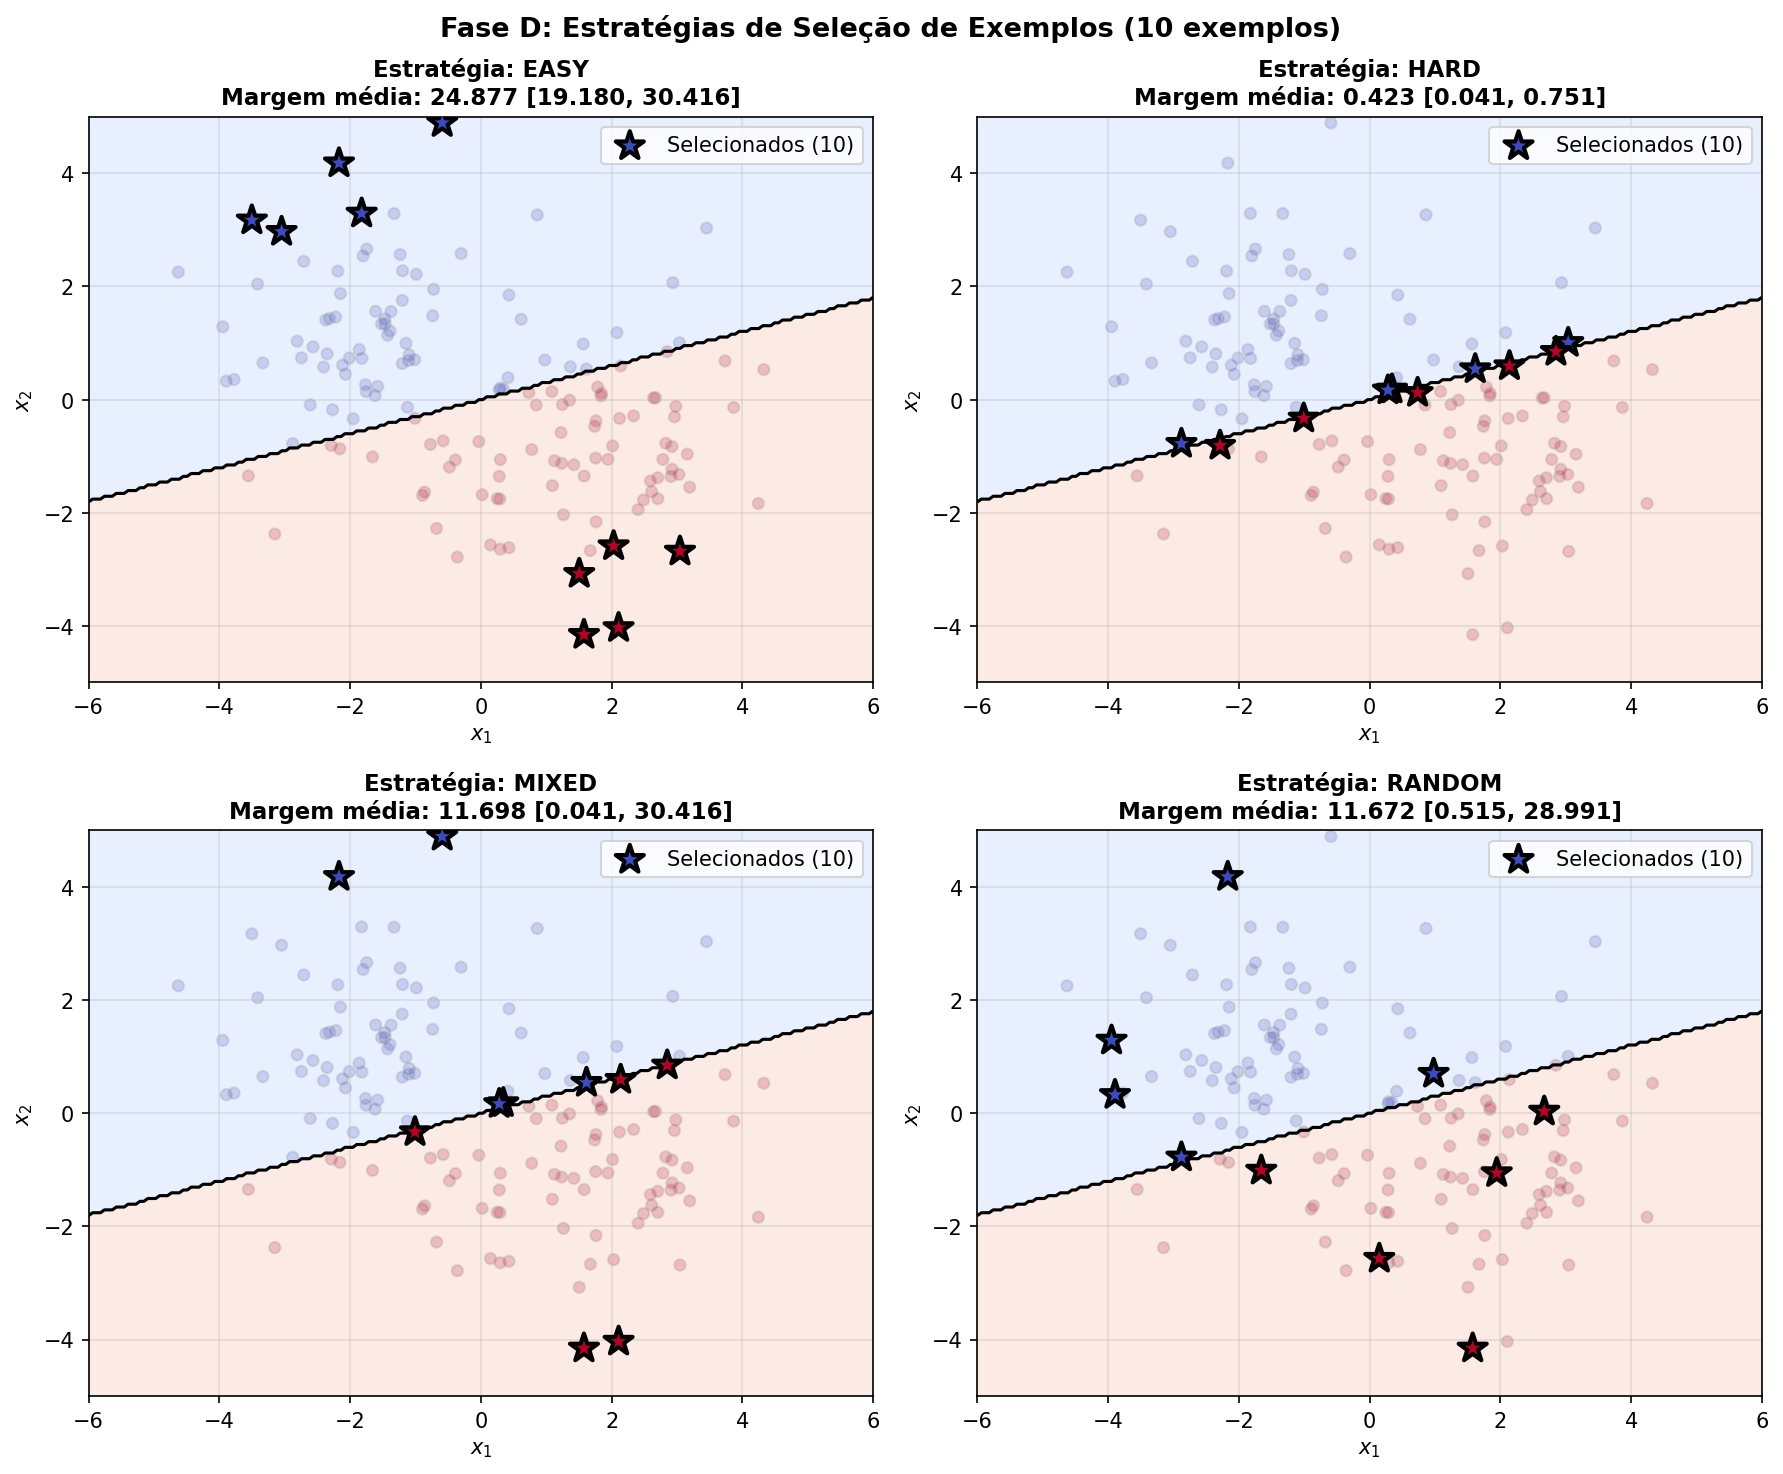
\includegraphics[width=0.78\linewidth,height=0.42\textheight,keepaspectratio]{07_phase_d_example_strategies.png}
  \end{center}
\end{frame}

% ============ SLIDE 32 ============
\begin{frame}{Fase D --- Curvas de Aprendizado}
  \scriptsize
  \textbf{Acur\'acia m\'edia LLM vs.\ perito (expert $=$ aniso\_x2, 3 seeds, 3 reps):}
  \begin{center}
  \begin{tabular}{rcccc}
    \toprule
    $\mathbf{n\_shot}$ & \textbf{easy} & \textbf{hard} & \textbf{mixed} & \textbf{random} \\
    \midrule
    0  & $60.9\%$ & $60.9\%$ & $60.9\%$ & $60.9\%$ \\
    5  & $85.8\%$ & $62.5\%$ & $82.0\%$ & $84.9\%$ \\
    10 & $86.9\%$ & $67.4\%$ & $79.4\%$ & $88.2\%$ \\
    20 & $90.2\%$ & $84.7\%$ & $86.9\%$ & $92.1\%$ \\
    40 & $88.0\%$ & $\mathbf{97.7\%}$ & $96.6\%$ & $94.0\%$ \\
    \bottomrule
  \end{tabular}
  \end{center}
  \vspace{-0.1cm}
  \begin{center}
    
\includegraphics[width=0.62\linewidth,height=0.38\textheight,keepaspectratio]{08_phase_d_learning_curve_accuracy.png}
  \end{center}
\end{frame}

% ============ SLIDE 33 ============
\begin{frame}{Fase D --- Compara\c{c}\~ao de Estrat\'egias}
  \begin{center}
    
\includegraphics[width=0.9\linewidth,height=0.72\textheight,keepaspectratio]{09_phase_d_strategy_comparison.png}
  \end{center}
  \scriptsize
  Melhor estrat\'egia por \texttt{n\_shot}: 5-shot = \textbf{random} ($84.1\%$); 10-shot = \textbf{random} ($89.2\%$); 20-shot = \textbf{random} ($93.1\%$); 40-shot = \textbf{hard} ($96.0\%$).
\end{frame}

% ============ SLIDE 34 ============
\begin{frame}{Refuta\c{c}\~ao de H4 --- Por que ``easy'' vence ``hard''?}
  \footnotesize
  \textbf{Acur\'acia m\'edia por estrat\'egia (todos $n > 0$):}
  \begin{center}
  \begin{tabular}{lc}
    \toprule
    \textbf{Estrat\'egia} & \textbf{Acur\'acia m\'edia} \\
    \midrule
    random & $\mathbf{90.3\%}$ \\
    mixed  & $87.8\%$ \\
    easy   & $81.5\%$ \\
    hard   & $75.6\%$ \\
    \bottomrule
  \end{tabular}
  \end{center}
  \medskip

  \textbf{Resultado:} H4 \textbf{refutada}. \emph{Exemplos easy ($81.5\%$) superam hard ($75.6\%$) consistentemente.}
  \medskip

  \textbf{Interpreta\c{c}\~ao proposta:}
  \begin{itemize}
    \item Exemplos pr\'oximos \`a fronteira s\~ao \emph{amb\'iguos} --- n\~ao fornecem padr\~oes claros de cada classe ao LLM.
    \item Exemplos f\'aceis funcionam como \emph{\^ancoras prototípicas}, definindo bem as regi\~oes de cada classe.
    \item Diferen\c{c}a conceitual com active learning em redes treinadas por gradiente: l\'a, exemplos dif\'iceis s\~ao mais informativos \emph{porque alteram os pesos}. Em LLMs com few-shot, o ``aprendizado'' \'e condicionamento, n\~ao atualiza\c{c}\~ao.
  \end{itemize}
\end{frame}

% ============ SLIDE 35 ============
\begin{frame}{Fase D --- M\'ultiplos Experts}
  \footnotesize
  \textbf{Acur\'acia m\'edia do LLM vs.\ perito (m\'edia sobre todas estrat\'egias e $n$'s, exceto zero-shot):}
  \begin{center}
  \begin{tabular}{llc}
    \toprule
    \textbf{Expert} & $W_{\text{expert}}$ & \textbf{Acur\'acia m\'edia} \\
    \midrule
    \texttt{aniso\_x2} ($x_2$ dominante) & $[0.3, 1.5]$ & $85.4\% \pm 10.9\%$ \\
    \texttt{aniso\_x1} ($x_1$ dominante) & $[1.5, 0.3]$ & $83.4\% \pm 13.9\%$ \\
    \texttt{euclidean} (pesos iguais)    & $[1.0, 1.0]$ & $82.5\% \pm 13.4\%$ \\
    \bottomrule
  \end{tabular}
  \end{center}
  \medskip

  \textbf{Interpreta\c{c}\~ao:} o LLM consegue aprender os 3 crit\'erios geom\'etricos distintos com desempenho similar $\Rightarrow$ a capacidade de aprendizado \textbf{n\~ao depende} da anisotropia espec\'ifica do perito. Evid\^encia forte para H3.
\end{frame}

% ============ SLIDE 36 ============
\begin{frame}{Experimento de Dilui\c{c}\~ao}
  \footnotesize
  \textbf{Design:} 4 exemplos \emph{hard} fixos $+$ $n$ exemplos \emph{easy} progressivos ($n \in \{0, 2, 4, 10, 16, 20\}$).
  \medskip

  \textbf{Pergunta:} os f\'aceis ``diluem'' os dif\'iceis e a performance deteriora?
  \vspace{-0.1cm}
  \begin{center}
    
\includegraphics[width=0.62\linewidth,height=0.52\textheight,keepaspectratio]{12_dilution_experiment_accuracy.png}
  \end{center}
  \scriptsize
  \textbf{Achado:} performance \textbf{aumenta monotonicamente} com mais easy ($57\% \to 86\%$). N\~ao h\'a dilui\c{c}\~ao --- pelo contr\'ario, os easy \emph{compensam} a ambiguidade dos hard. Consistente com a refuta\c{c}\~ao de H4.
\end{frame}

% ============ SLIDE 37 ============
\begin{frame}{Vi\'es de Ordem dos Exemplos Few-Shot (Recency Bias)}
  \scriptsize
  \textbf{4 ordena\c{c}\~oes} dos mesmos exemplos (estrat\'egia mixed):
  \begin{center}
  \begin{tabular}{lccc}
    \toprule
    \textbf{Ordena\c{c}\~ao} & \textbf{5-shot} & \textbf{10-shot} & \textbf{20-shot} \\
    \midrule
    alternating   & $82.0\%$ & $85.1\%$ & $87.3\%$ \\
    class0\_first & $82.0\%$ & $80.0\%$ & $86.2\%$ \\
    class1\_first & $78.5\%$ & $83.1\%$ & $85.6\%$ \\
    shuffled      & $80.7\%$ & $87.3\%$ & $85.6\%$ \\
    \bottomrule
  \end{tabular}
  \end{center}
  \medskip

  \textbf{Testes de Kruskal-Wallis por $n\_shot$:}
  \begin{itemize}
    \item 5-shot:  $H = 0.560$, $p = 0.905$ --- n\~ao significativo
    \item 10-shot: $H = 4.741$, $p = 0.192$ --- n\~ao significativo
    \item 20-shot: $H = 1.171$, $p = 0.760$ --- n\~ao significativo
  \end{itemize}
  \medskip

  \textbf{Resultado:} varia\c{c}\~ao total $< 3$ p.p.\ $\Rightarrow$ \textbf{recency bias negligenci\'avel} na faixa testada.
\end{frame}

% ============ SLIDE 38 ============
\begin{frame}{Valida\c{c}\~ao Oracle --- Recupera\c{c}\~ao de W}
  \footnotesize
  \textbf{Sanity check:} gerar dados sint\'eticos com $W_{\text{gt}}$ conhecido, rotular com $W_{\text{gt}}$, e verificar se os 3 algoritmos recuperam $W_{\text{gt}}$.
  \medskip

  \textbf{Configs testadas} (seed 42, Problema D):
  \begin{center}
  \begin{tabular}{llccc}
    \toprule
    \textbf{Config} & $W_{\text{gt}}$ & \textbf{Perceptron} & \textbf{NNLS} \\
     & & $\cos(W_{\text{rec}}, W_{\text{gt}})$ & $\cos$ \\
    \midrule
    aniso\_x2    & $[0.3, 1.5]$       & $\mathbf{0.9999}$ & $0.9933$ \\
    aniso\_x1    & $[1.5, 0.3]$       & $0.9979$ & $0.9894$ \\
    euclidean    & $[1.0, 1.0]$       & $0.9990$ & $0.9960$ \\
    forte\_aniso & $[11.1, 0.44]$ & $0.9999$ & $0.9999$ \\
    \bottomrule
  \end{tabular}
  \end{center}
  \medskip

  \textbf{Resultado:} os 2 algoritmos recuperam $W_{\text{gt}}$ com $\cos \geq 0.98$ em todas as configs anisotrópicas $\Rightarrow$ \textbf{piso de sanidade confirmado}. Falhas em dados reais do LLM n\~ao s\~ao falhas dos algoritmos.
\end{frame}

% ============ SLIDE 39 ============
\begin{frame}{Valida\c{c}\~ao Oracle --- Transfer\^encia entre Geometrias}
  \footnotesize
  \textbf{Experimento:} aprender $W$ em uma geometria ($x_2\_dom$) e aplicar em outras ($x_1\_dom$, $forte\_aniso$).
  \vspace{-0.1cm}
  \begin{center}
    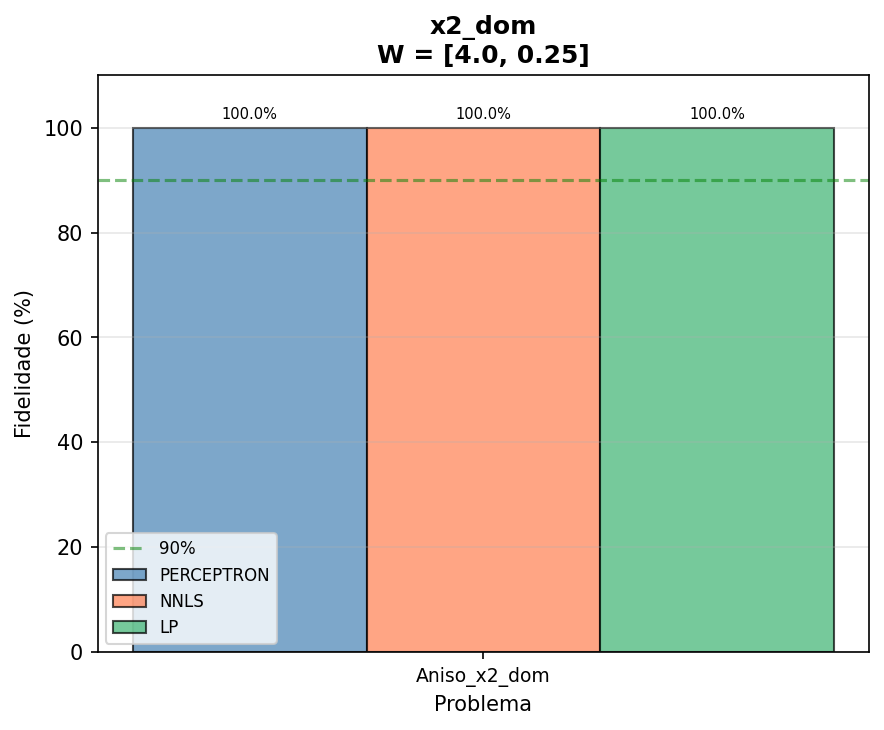
\includegraphics[width=0.6\linewidth,height=0.48\textheight,keepaspectratio]{23_oracle_transfer_x2_dom.png}
  \end{center}
  \medskip

  \textbf{Achado:} quando a geometria muda, a consist\^encia \textbf{cai drasticamente} --- $W$ ``aprendido'' em uma geometria \emph{n\~ao \'e universal}. A m\'etrica \'e \emph{acoplada} aos centr\'oides do problema. Implica\c{c}\~ao para H1: inconsist\^encia cross-problem reflete desalinhamento geom\'etrico, n\~ao necessariamente variabilidade do LLM.
\end{frame}

% ============ SLIDE 40 ============
\begin{frame}{Proje\c{c}\~ao R3 --- Metodologia}
  \footnotesize
  \textbf{Motiva\c{c}\~ao:} a m\'etrica diagonal \'e limitada --- n\~ao captura intera\c{c}\~oes entre features. \\
  \textbf{Solu\c{c}\~ao:} adicionar uma \emph{terceira feature} $x_3 = x_1 \cdot x_2$ (kernel quadr\'atico impl\'icito).
  \medskip

  \textbf{Nova m\'etrica:}
  \[
    d_W(x, c) = w_1 (x_1 - c_1)^2 + w_2 (x_2 - c_2)^2 + w_3 (x_3 - c_3)^2
  \]

  \textbf{Protocolo de compara\c{c}\~ao:}
  \begin{enumerate}
    \item LLM classifica com 2 features (baseline).
    \item LLM classifica com 3 features (agora $x_1, x_2, x_3$).
    \item Cada um dos 3 algoritmos aprende $W \in \mathbb{R}^3$.
    \item Reportar fidelidade e peso de $x_3$ --- se $w_3 > 0$, a intera\c{c}\~ao importa.
  \end{enumerate}
\end{frame}

% ============ SLIDE 41 ============
\begin{frame}{Proje\c{c}\~ao R3 --- Resultados}
  \scriptsize
  \textbf{Fidelidade (3 seeds, m\'edia):}
  \begin{center}
  \begin{tabular}{lcccc}
    \toprule
    \textbf{Condi\c{c}\~ao} & \textbf{Algoritmo} & \textbf{Fid.} & $\hat{W}$ & \textbf{Peso de} $x_3$ \\
    \midrule
    LLM 2 features & --- & $84.4\%$ & --- & --- \\
    \midrule
    LLM 3 features + Perceptron & Perceptron & $75.1\%$ & $[0.2, 0.6, 0.1]$ & $\sim 8\%$ \\
    LLM 3 features + NNLS       & NNLS       & $86.2\%$ & $[0.04, 0.15, 0.02]$ & $\sim 8\%$ \\
    \bottomrule
  \end{tabular}
  \end{center}
  \vspace{-0.05cm}
  \begin{center}
    
\includegraphics[width=0.55\linewidth,height=0.42\textheight,keepaspectratio]{13_r3_vs_r2_linear_vs_quadratica.png}
  \end{center}
  \scriptsize
  \textbf{Achado:} adicionar $x_3$ \textbf{n\~ao melhora} significativamente a fidelidade $\Rightarrow$ LLM n\~ao captura intera\c{c}\~ao quadr\'atica neste problema. M\'etrica diagonal linear \'e suficiente.
\end{frame}

% ============ SLIDE 42 ============
\begin{frame}{Baselines Cl\'assicos --- Configura\c{c}\~ao}
  \footnotesize
  \textbf{3 classificadores} treinados nos \textbf{mesmos exemplos few-shot} da Fase D e avaliados no \textbf{mesmo conjunto de teste}:
  \begin{description}
    \item[\textbf{k-NN}] \texttt{sklearn.KNeighborsClassifier}, $k = \min(5, n\_shot)$, ajustado \'impar.
    \item[\textbf{Logistic Regression}] regulariza\c{c}\~ao L2, \texttt{max\_iter = 1000}.
    \item[\textbf{SVM (RBF)}] \texttt{sklearn.SVC(kernel='rbf')}, par\^ametros padr\~ao.
  \end{description}
  \medskip

  \textbf{Pergunta:} o LLM faz algo que um classificador trivial \emph{n\~ao} faria com os mesmos dados? Se baselines superam o LLM no few-shot $\Rightarrow$ o LLM n\~ao est\'a agregando informa\c{c}\~ao.
\end{frame}

% ============ SLIDE 43 ============
\begin{frame}{Baselines Cl\'assicos --- Resultados}
  \scriptsize
  \textbf{Acur\'acia m\'edia vs.\ perito (todos $n\_shot$, todas estrat\'egias):}
  \begin{center}
  \begin{tabular}{lcc}
    \toprule
    \textbf{Modelo} & \textbf{Acur\'acia m\'edia} & \textbf{Kappa} \\
    \midrule
    LLM (melhor config)  & $\approx 96\%$ & $\approx 0.92$ \\
    Logistic Regression  & $93.4\%$ & $0.868$ \\
    SVM (RBF)            & $87.5\%$ & $0.750$ \\
    k-NN ($k=5$)         & $89.5\%$ & $0.790$ \\
    k-NN ($k=3$)         & $84.0\%$ & $0.684$ \\
    \bottomrule
  \end{tabular}
  \end{center}
  \vspace{-0.1cm}
  \begin{center}
    
\includegraphics[width=0.55\linewidth,height=0.4\textheight,keepaspectratio]{18_classical_baselines_accuracy.png}
  \end{center}
  \scriptsize
  \textbf{Conclus\~ao:} LLM \emph{n\~ao \'e dominado} por baselines; Logistic Regression \'e o mais pr\'oximo. A vantagem do LLM est\'a em robustez semântica, n\~ao em acur\'acia pura.
\end{frame}

% ============ SLIDE 44 ============
\begin{frame}{Robustez entre Seeds}
  \begin{center}
    
\includegraphics[width=0.88\linewidth,height=0.75\textheight,keepaspectratio]{05_seed_comparison.png}
  \end{center}
  \scriptsize
  Consist\^encia entre seeds (agregada): m\'edia $76.9\%$, desvio $\pm 13\%$; cosseno m\'edio entre $W$s $= 0.984$. H5 \textbf{sustentada} --- comportamento reprodut\'ivel.
\end{frame}

% ============ SLIDE 45 ============
\begin{frame}{Testes Estat\'isticos Principais}
  \footnotesize
  \textbf{Bootstrap 95\% CI (10k reamostras), Fases A-C (classes A/B, default prompt):}
  \begin{center}
  \begin{tabular}{lcc}
    \toprule
    \textbf{M\'etrica} ($n\_shot$) & \textbf{M\'edia} & \textbf{CI$_{95}$} \\
    \midrule
    Fidelidade A (Perc, $n=0$)          & $0.813$ & $[0.762, 0.845]$ \\
    Consist\^encia B (Perc, $n=0$)      & $0.724$ & $[0.677, 0.765]$ \\
    Consist\^encia B (Perc, $n=10$)     & $0.810$ & $[0.770, 0.851]$ \\
    Kappa B (Perc, $n=10$)              & $0.612$ & $[0.536, 0.689]$ \\
    Kappa C (NNLS, $n=20$)              & $0.530$ & $[0.393, 0.666]$ \\
    \bottomrule
  \end{tabular}
  \end{center}

  \textbf{Teste: Zero-shot vs.\ 10-shot (Wilcoxon pareado, Cohen's d):}
  \begin{itemize}
    \item Consist.\ B: $\Delta = +7.7$ p.p., CI$_{95}$ $[+6.1, +10.0]$, $d = 1.29$ (\emph{grande})
    \item Consist.\ C: $\Delta = -3.6$ p.p., CI$_{95}$ $[-15.9, +3.7]$, $d = -0.72$ (\emph{m\'edio})
  \end{itemize}

  \textbf{Teste: M\'etrica vs.\ Euclidiana (zero-shot, B):} $\Delta = +14.8$ p.p., CI$_{95}$ $[+3.5, +30.4]$ $\Rightarrow$ \textbf{significativo}.
\end{frame}

% ============ SLIDE 46 ============
\begin{frame}{Testes Estat\'isticos Complementares}
  \footnotesize
  \textbf{Testes n\~ao-param\'etricos adicionais:}
  \medskip

  \textbf{1. Correla\c{c}\~ao ponto-bisserial} (acerto do LLM $\times$ margem do ponto, Fase A):
  \begin{itemize}
    \item Seed 42: $r = 0.395$, $p < 0.001$
    \item Seed 7:  $r = 0.438$, $p < 0.001$
    \item Seed 123: $r = 0.232$, $p = 0.004$
  \end{itemize}
  $\Rightarrow$ \emph{Correla\c{c}\~ao positiva significativa entre margem e acerto em todas as seeds.}
  \medskip

  \textbf{2. Mann-Whitney U} (margem de acertos $>$ margem de erros):
  \begin{itemize}
    \item Seed 42: $U = 2708$, $p < 0.001$
    \item Seed 7:  $U = 2806$, $p < 0.001$
    \item Seed 123: $U = 1834$, $p = 0.002$
  \end{itemize}
  $\Rightarrow$ \emph{Erros concentram-se em pontos com baixa margem, confirmado em todas as seeds.}
  \medskip

  \textbf{3. Kruskal-Wallis} (ordem dos exemplos few-shot):
  \begin{itemize}
    \item 5-shot: $H = 0.56$, $p = 0.91$; 10-shot: $H = 4.74$, $p = 0.19$; 20-shot: $H = 1.17$, $p = 0.76$.
  \end{itemize}
  $\Rightarrow$ \emph{Ordem dos exemplos N\~AO afeta performance (recency bias ausente).}
\end{frame}

% ============ SLIDE 47 ============
\begin{frame}{Dashboards Explorat\'orios por Seed}
  \begin{center}
    
\includegraphics[width=0.85\linewidth,height=0.80\textheight,keepaspectratio]{19_experiment_dashboard_seed42.png}
  \end{center}
  \scriptsize
  Dashboard consolidado (seed 42): distribui\c{c}\~ao de $W$, matrizes de confus\~ao, curvas de aprendizado e compara\c{c}\~ao entre algoritmos em uma \'unica vista.
\end{frame}

% ============ SLIDE 48 ============
\begin{frame}{S\'intese das Hip\'oteses}
  \footnotesize
  \begin{center}
  \begin{tabular}{clp{5.5cm}c}
    \toprule
    \textbf{Hip.} & \textbf{Descri\c{c}\~ao} & \textbf{Evid\^encia} & \textbf{Veredito} \\
    \midrule
    H1 & Consist\^encia & Consist.\ B $= 78\%$, C $= 76\%$; Kappa em $[0.4, 0.7]$ & \color{orange}Parcial \\
    H2 & Few-shot amplifica & $\Delta = +7.7$ p.p., $d = 1.29$ (zero vs 10-shot, B) & \color{green!70!black}Confirmada \\
    H3 & LLM como aprendiz & Fase D: $55\% \to 96\%$ com 40-shot (qualquer expert) & \color{green!70!black}Confirmada \\
    H4 & Hard mais informativo & Easy ($82\%$) $>$ Hard ($76\%$); random $= 90\%$ & \color{red!80!black}Refutada \\
    H5 & Estabilidade & $\cos$ entre seeds $= 0.984$; CV da raz\~ao $= 6\%$ em $n \geq 5$ & \color{green!70!black}Confirmada \\
    \bottomrule
  \end{tabular}
  \end{center}
  \medskip

  \textbf{Destaque:} H4 refutada \'e o achado mais original --- contradiz a intui\c{c}\~ao de active learning e sugere que few-shot em LLMs funciona por \emph{condicionamento prototípico}, n\~ao por \emph{atualiza\c{c}\~ao de pesos}.
\end{frame}

% ============================================================
% ADENDOS APÓS REUNIÃO 30/04/2026 — SLIDES NOVOS
% ============================================================

% ============ Prompts literais (1/2) ============
\begin{frame}[fragile]{Prompts literais (1/2) --- zero-shot e few-shot default}
  \tiny
  \textbf{Prompt zero-shot (default):}
\begin{verbatim}
You are a binary classifier for 2D points.

Classify the given point as Class A or Class B.
Answer ONLY with "A" or "B", nothing else.

Point to classify:
x1 = -1.4321
x2 = 0.8932

Your classification:
\end{verbatim}

  \textbf{Prompt few-shot (default, 5 exemplos):}
\begin{verbatim}
You are a binary classifier for 2D points.
Learn the classification pattern from the examples below, then classify the new point.

Examples:
  x1 = -1.5000, x2 = 1.0000 -> A
  x1 =  1.5000, x2 = -1.0000 -> B
  x1 = -1.2000, x2 = 0.5000 -> A
  x1 =  1.0000, x2 = -0.7000 -> B
  x1 = -0.8000, x2 = 0.9000 -> A

Answer ONLY with "A" or "B", nothing else.

Point to classify:
x1 = -1.4321
x2 = 0.8932

Your classification:
\end{verbatim}
\end{frame}

% ============ Prompts literais (2/2) ============
\begin{frame}[fragile]{Prompts literais (2/2) --- variantes geometric / CoT / tabular}
  \tiny
  \textbf{Geometric:} adiciona contexto espacial ao default
\begin{verbatim}
You are a binary classifier for 2D points represented as (x1, x2) coordinates
in a plane. The boundary between classes is geometric.
Classify ... [resto igual ao default]
\end{verbatim}

  \textbf{Chain-of-thought (CoT):} pede racioc\'inio passo a passo
\begin{verbatim}
You are a binary classifier for 2D points.
Think step by step about which class is closer based on the examples, then answer.

Examples: ...
Point: x1=-1.4321, x2=0.8932

Reasoning (be brief), then final answer "A" or "B":
\end{verbatim}

  \textbf{Tabular:} coordenadas como tabela markdown
\begin{verbatim}
| x1     | x2     | class |
|--------|--------|-------|
| -1.5   |  1.0   | A     |
|  1.5   | -1.0   | B     |
| ...                     |

Classify | -1.4321 | 0.8932 | ? |
\end{verbatim}
\end{frame}

% ============ Transição: BLOCO II (LLM como aprendiz) ============
\begin{frame}{Bloco II --- LLM como APRENDIZ (in-context learning)}
  \footnotesize
  \begin{itemize}
    \item Os pap\'eis se invertem: um \emph{perito} (expert ou m\'etrica ora\'culo) rotula os dados; o LLM tenta \emph{reproduzir} essas decis\~oes via few-shot.
    \item Cobre Fase D (sint\'etico anisotr\'opico), peso $\times$ altura (real, fronteira el\'iptica), meia-lua (sint\'etico n\~ao-linear).
    \item Hip\'oteses ligadas a este bloco:
      \begin{itemize}
        \item \textbf{H3} — LLM \'e capaz de aprender crit\'erio externo via few-shot.
        \item \textbf{H4} — exemplos dif\'iceis ensinam mais (\textbf{REFUTADA}).
        \item \textbf{H5} — estabilidade entre seeds (transversal).
      \end{itemize}
  \end{itemize}
\end{frame}

% ============ Parte 2: peso × altura (placeholder até nova execução) ============
\begin{frame}{Estudo de caso real --- peso $\times$ altura (homem/mulher)}
  \footnotesize
  \textbf{Base enviada pelo orientador} (e-mail 30/04/2026 19:15):
  \begin{itemize}
    \item $\sim$100 amostras normalizadas em $[-1, 1]$, balanceado 50/50.
    \item Classificador \'otimo bayesiano: \emph{elipse}
    \[
      f(x_1, x_2) = x_2^2 - x_2 + x_1^2 - x_1 + \text{cte}
    \]
    (fronteira quadr\'atica).
  \end{itemize}
  \medskip

  \textbf{Protocolo (e-mail 22:04):}
  \begin{itemize}
    \item Repetir apenas Fases A e D nesta base.
    \item Variantes de prompt: $(x_1, x_2)$ neutro vs.\ $(\text{peso}, \text{altura})$ sem\^antico.
    \item Pergunta: classificar como \textbf{Homem} ou \textbf{Mulher}.
    \item Fase A com 2 / 3 / 4 features:
      \begin{itemize}
        \item 2: $(x_1, x_2)$
        \item 3 (hip\'erbole): $(x_1, x_2, x_1 \cdot x_2)$
        \item 4 (elipse): $(x_1, x_2, x_1^2, x_2^2)$
      \end{itemize}
    \item Reportar fidelidade vs.\ LLM \textbf{e} acur\'acia vs.\ r\'otulo real.
    \item Identificar melhor $n$-features e rodar Fase D com essa m\'etrica.
  \end{itemize}
  \medskip

  \textit{\small Resultados num\'ericos ser\~ao preenchidos ap\'os a pr\'oxima execu\c{c}\~ao com \texttt{RUN\_HOMEM\_MULHER=True}.}
\end{frame}

% ============ Parte 3: meia-lua (placeholder até nova execução) ============
\begin{frame}{Problema E --- meia-lua (sint\'etico n\~ao-linear)}
  \footnotesize
  \textbf{Justificativa} (reuni\~ao $\sim$2558s): o experimento R3 em A/B/C \emph{lineares} n\~ao melhorou ao adicionar $x_1 \cdot x_2$ (84\% $\to$ 75\%). Aqui sim --- a meia-lua \'e \emph{genuinamente n\~ao-linear}.
  \medskip

  \textbf{Setup:}
  \begin{itemize}
    \item \texttt{sklearn.datasets.make\_moons(n\_samples=150, noise=0.15)}.
    \item Pergunta: classificar como classe A ou B.
    \item Fase A com 2 / 3 / 4 features (mesmas configura\c{c}\~oes da Parte 2).
    \item Fase D com a melhor m\'etrica.
  \end{itemize}
  \medskip

  \textbf{Expectativa} (orientador $\sim$2740s):
  \begin{quote}
    ``Se o problema \'e linear, matematicamente ele n\~ao vai melhorar [...]
    Agora se o problema \'e mais dif\'icil, de repente se com a outra
    componente a gente conseguir melhorar a m\'etrica, \'e sinal de que ela
    capturou uma n\~ao linearidade na estrat\'egia do LLM.''
  \end{quote}
  \medskip

  \textit{\small Resultados num\'ericos ser\~ao preenchidos ap\'os a pr\'oxima execu\c{c}\~ao com \texttt{RUN\_PROBLEM\_E=True}.}
\end{frame}

% ============ Comparação cruzada linear × não-linear ============
\begin{frame}{Compara\c{c}\~ao cruzada --- linear $\times$ n\~ao-linear}
  \footnotesize
  Tabela consolidada de ganhos ao passar de 2 $\to$ 3 $\to$ 4 features:
  \medskip

  \begin{center}
  \begin{tabular}{lccc}
    \toprule
    \textbf{Problema} & \textbf{Tipo} & \textbf{Ganho 2$\to$3 feat.} & \textbf{Ganho 2$\to$4 feat.} \\
    \midrule
    A / B / C (gaussianas) & Linear        & $\sim 0\%$ (refer\^encia atual) & --- \\
    Meia-lua               & N\~ao-linear  & a preencher                     & a preencher \\
    Peso $\times$ altura   & N\~ao-linear (elipse) & a preencher              & a preencher \\
    \bottomrule
  \end{tabular}
  \end{center}
  \medskip

  \textbf{Hip\'otese de trabalho}: ganho apenas em problemas n\~ao-lineares.
  Em problemas lineares, a m\'etrica diagonal 2D j\'a representa a fronteira
  --- adicionar features quadr\'aticas n\~ao ajuda. Em problemas n\~ao-lineares,
  features quadr\'aticas s\~ao necess\'arias para a m\'etrica diagonal capturar a fronteira.
  \medskip

  \textbf{Citação orientador (\textasciitilde2843s):} \emph{``Eu acho que a gente fecha at\'e um artigo j\'a''}.
\end{frame}

% ============ SLIDE Final ============
\begin{frame}
  \begin{center}
    \Huge Obrigado!
    \medskip

    \Large Perguntas?
    \vspace{2cm}

    \normalsize
    George Gomes da Silva \\
    \texttt{georgegomesdasil@gmail.com}
  \end{center}
\end{frame}

\end{document}
